\documentclass[conference]{IEEEtran}
\IEEEoverridecommandlockouts
% The preceding line is only needed to identify funding in the first footnote. If that is unneeded, please comment it out.
\usepackage{cite}
\usepackage{algorithmic}
\usepackage{graphicx}
\usepackage{textcomp}
\usepackage{amsmath}
\usepackage[sc]{mathpazo}
\usepackage{datetime}
\usepackage{graphicx, wrapfig, subcaption, setspace, booktabs}
\usepackage[T1]{fontenc}
\usepackage{fourier}
\usepackage{url, lipsum}
\usepackage{hyperref,bookmark}
\usepackage[T1]{fontenc}
\usepackage{amssymb}
\usepackage{makecell, multirow, tabularx}
\usepackage{listings}
\usepackage[ruled,linesnumbered,vlined]{algorithm2e}

\usepackage{float}
\usepackage{nomencl}
\usepackage{ifthen}

\renewcommand{\nomgroup}[1]{%
	\ifthenelse{\equal{#1}{P}}{\item[\textbf{Parameters}]}{%
		\ifthenelse{\equal{#1}{V}}{\item[\textbf{Variables \\}]}}
}
\makenomenclature
\def\BibTeX{{\rm B\kern-.05em{\sc i\kern-.025em b}\kern-.08em
    T\kern-.1667em\lower.7ex\hbox{E}\kern-.125emX}}
\begin{document}

\title{CO\textsubscript{2} Impact Electric Vehicle Charging on a Local Microgrid: a case study in Southern California }
%\Thanks{Identify Applicable Funding Agency Here. If None, Delete This.}
%}
%

%\author{\IEEEauthorblockN{1\textsuperscript{st}  Luis Fernando Enriquez-Contreras, Jacqueline Garrido,  Matthew Barth, Sadrul Ula, Arun Raju}
%	\IEEEauthorblockA{\textit{Department of Electrical  and Computer Engineering} \\
%		\textit{University of California, Riverside}\\
%		Riverside, United States of America \\
%		lenri001@ucr.edu, jgarr023@ucr.edu, barth@ece.ucr.edu, sula@cert.ucr.edu,  arun@engr.ucr.edu  }
%	\and
%	\IEEEauthorblockN{2\textsuperscript{nd} A S M Jahid Hasan}
%	\IEEEauthorblockA{\textit{Department of Electrical and Computer Engineering} \\
%		\textit{North South University}\\
%		Dhaka, Bangladesh\\
%		jahid.hasan12@northsouth.edu }
%	\and
%	\IEEEauthorblockN{3\textsuperscript{rd} Jubair Yusuf}
%	\IEEEauthorblockA{\textit{Electric Power Systems Research} \\
%		\textit{Sandia National Laboratories}\\
%		Albuquerque,  United States of America\\
%		jyusuf@sandia.gov}
%
%
%}

\author{
	\IEEEauthorblockN{1\textsuperscript{st} Luis Fernando Enriquez-Contreras\IEEEauthorrefmark{1}\IEEEauthorrefmark{2}, Jacqueline Garrido\IEEEauthorrefmark{1}\IEEEauthorrefmark{2}, Matthew Barth\IEEEauthorrefmark{1}\IEEEauthorrefmark{2}, Sadrul Ula\IEEEauthorrefmark{2}, Arun Raju\IEEEauthorrefmark{2}}
	\IEEEauthorblockA{\IEEEauthorrefmark{1}\textit{Department of Electrical  and Computer Engineering} \\
		\textit{University of California, Riverside}\\
				Riverside, United States of America \\
				lenri001@ucr.edu, jgarr023@ucr.edu, barth@ece.ucr.edu}
	\IEEEauthorblockA{\IEEEauthorrefmark{2}\textit{College of Engineering, Center for Environmental Research \& Technology} \\
		\textit{University of California, Riverside}\\
				Riverside, United States of America \\
				lenri001@ucr.edu, jgarr023@ucr.edu, barth@ece.ucr.edu, sula@cert.ucr.edu,  arun@engr.ucr.edu}
		\and
	\IEEEauthorblockN{2\textsuperscript{nd} A S M Jahid Hasan}
	\IEEEauthorblockA{\textit{Department of Electrical and Computer Engineering} \\
			\textit{North South University}\\
			Dhaka, Bangladesh\\
			jahid.hasan12@northsouth.edu }
		\and
	\IEEEauthorblockN{3\textsuperscript{rd} Jubair Yusuf}
	\IEEEauthorblockA{\textit{Department of Electrical  and Computer Engineering} \\
			\textit{University of California, Riverside}\\
			Riverside,  United States of America\\
			jyusu001@ucr.edu}
}
\maketitle

\begin{abstract}

		As renewable energy penetration in electric grids increases with time, it becomes more important for electric utilities to update their electric rates  such that they minimize CO\textsubscript{2} emissions. In this paper, we evaluate a case study at the University of California, Riverside (UCR) to simulate different Time of Use (TOU) rate optimizations that minimizes electric costs while analyzing CO\textsubscript{2} output, by using the openmodelica model, we based on different electric utility rates in Southern California.  The different amounts of power and energy consumed by each rate is compared with CAISO CO\textsubscript{2} emissions data in order to review the different emission levels from the different utility electric rates on a 15 minute basis.  Electric costs are also compared in order to see the different savings the consumer will have with the different rates. It was found that Southern California Edison (SCE) TOU rate had the most savings for the consumer and that Riverside (RPU) TOU flat rate had the lowest CO\textsubscript{2} emissions.

\end{abstract}

\begin{IEEEkeywords}
micorgrids, demand response, TOU, CO\textsubscript{2} emissions, modelica
\end{IEEEkeywords}

%Parameters

%\nomenclature[P0]{$t$}{Timestep in seconds}
%
%\nomenclature[P1]{$\Delta t$}{Duration of each timestep}
%
%\nomenclature[P2]{$T^{\prime}$}{Total number of timesteps}
%
%\nomenclature[P3]{$E_{\text {init }}^{B}$}{Initial stored energy of the BESS}
%
%\nomenclature[P4]{$P_{t}^{S}$}{Solar generation $\mathrm{t}$}
%
%\nomenclature[P5]{$P_{t}^{L}$}{Load at $\mathrm{t}$}
%
%\nomenclature[P6]{$\alpha_{t}$}{Energy charge at $\mathrm{t}$}
%
%\nomenclature[P7]{$\beta$}{Monthly peak demand charge}
%
%\nomenclature[P8]{$\beta_{t}^{\text {On }} / \beta_{t}^{\text {Mid }} / \beta_{t}^{\text {Off }}$}{$\mathrm{On} / \mathrm{Mid} / $Off-Peak demand charges at $\mathrm{t}$}
%
%\nomenclature[P8]{$\eta^{+} / \eta^{-}$}{Charging/discharging efficiency of BESS}
%
%%Variables
%\nomenclature[Vx]{}{}
%\nomenclature[V0]{$E_{t}^{B}$}{Energy stored at $\mathrm{t}$ in BESS}
%
%\nomenclature[V1]{$P_{t}^{B}$}{BESS power at $\mathrm{t}$}
%
%\nomenclature[V2]{$P_{t}^{B+} / P_{t}^{B-}$}{BESS charging/discharging power at $\mathrm{t}$}
%
%\nomenclature[V3]{$P_{t}^{G}$}{Power drawn from the grid at $\mathrm{t}$}
%
%\nomenclature[V4]{$P_{t}^{S B}$}{Solar power fed to BESS at $\mathrm{t}$}
%
%\nomenclature[V5]{$P_{t}^{S L}$}{Solar power fed to load at $\mathrm{t}$}
%
%\nomenclature[V6]{$P_{t}^{B L}$}{BESS power fed to load at $\mathrm{t}$}
%
%\printnomenclature
\section{Introduction}
    \subsection{Background}
	California is committed to reducing greenhouse gas emissions through various approaches. However, the two largest contributors to greenhouse gas emissions in California are transportation and electricity generation. California currently has X percent of electric vehicle sales and plans on banning internal combustion engine vehicles by 2035. At the same time, California is increasing the number of charging stations in the state, having over X currently and Y amount in 20xx. Electric vehicle technology has improved, and new vehicles can charge in X minutes. This is due to Level 3 charging, which can be as high as 350 kilowatts (kW) opposed to Level 2 charging, which is capped at 19 kW. While this innovation has led to a higher practicality for electric vehicles, it also leads to more difficulty for the owners of these chargers since they can create a tremendous amount of loads very quickly. Most Level 2 chargers consumers use are similar in load to an air conditioner. While California tries to increase clean energy penetration, it also needs to reduce the amount of GHG emissions produced by transportation through electrification. This leads to two conundrums: how will California add enough capacity for electrified transport, and how clean is the grid to minimize the amount of emissions associated with battery electric vehicles? One proposal to mitigate the strain on the grid is to keep electricity production and EV charging local by using microgrids. A microgrid is defined as: “‘a group of interconnected loads and distributed energy resources within clearly defined electrical boundaries that acts as a single controllable entity with respect to the grid. A microgrid can connect and disconnect from the grid to enable it to operate in both grid-connected or island-mode” As microgrids and EV chargers become ubiquitous, it is crucial to study the economic and environmental impacts EV charging in particular fast charging, will have on microgrids.
  	\subsection{Literature Review}
  	In  \cite{himabindu2021analysis},   Electric Vehicle Charging Station (EVCS) are analyzed under different solar irradiation conditions.  A demand and stochastic model is devoloped, a techno-economic assessment is done, and the environmental impacts are analyzed.  The authors conclude that EVCS with solar's optimal configuration  and investment costs are highly dependent on feed-in tariffs and  the solar irradiation of the area. The  CO\textsubscript{2} emissions were calculated on a per years basis, and do not deal with the variations of  CO\textsubscript{2} emissions within a single day.  Also, only energy charges where calculated with bo demand costs calculations.  In \citen{yoon2017economic},  a control algorithm is proposed with that in different scenarios can minimize charging time or costs or maximize renewable energy use. The authors used a uniform distribution during peak times  to model the charging loads, and only level 2 charging at 3.3 kW no level 3 charging. An EV charging model is proposed in \cite{purvins2018electric},  that load shifts charging events from high peak times to low peak times.  The authors found their current method does little to reduce peak load shaving, and solar production surplus may not be necessarily shifted to EVs due to their low availability at the time.  The dataset was limited to one week , with four EVs in a system with 10 buildings.  In \cite{Khemir}, the author run multiple scenarios with different self consumption rates. The scenarios are compared and the CO\textsubscript{2} emissions for each scenario are calculated. The CO\textsubscript{2} emissions are calculated from a whole life-cycle CO \textsubscript{2}  emissions. 
  	
%			Previous literature has explored various topics concerning TOU impacts on  CO\textsubscript{2} emissions. In \cite{schedulingcontroller}, a lightning search algorithm (LSA) is used to optimize a microgrid controller based on CO\textsubscript{2} emissions, energy use, and demand costs. Their model predicts a reduction of 78 to 220 tons of CO\textsubscript{2} from the atmosphere, does not optimize using TOU rates, and calculates emissions using a flat demand. In \cite{economicandenvironmentalpolicy}, the authors investigate the deployment cost of multiple scenarios in a multi-carrier microgrid (MCMG) model that considers demand shifting, monthly peak, and CO\textsubscript{2} emissions. They advocate for better environmental policies in the utility sector since the MCMG scenario optimized solely for CO\textsubscript{2} emissions was 39\% less cost-effective than the scenario optimized for cost.  In  \cite{stochasticoptimalscheduling}, simulations are run on a system consisting of three microgrids while considering and neglecting emission charges. CO\textsubscript{2} Emissions were halved when considering CO\textsubscript{2} emissions charges. However, the lower emission operation has a higher upfront cost and is less economically attractive for customers. In \cite{emsformg} five scenarios with cost and emission reduction in mind are done in an isolated microgrid. The authors conclude that running the pareto control strategy is the best compromise between cost and CO\textsubscript{2} emissions output. The different case scenarios were different balances between cost and CO\textsubscript{2} emissions, but only used one electric rate. In \cite{abcdr}, the authors assess different demand side management strategies utilizing the Artificial Bee Colony algorithm under different tariff structures. TOU, critical peak pricing (CPP), real-time electricity pricing (RTEP), and day-ahead pricing (DAP) seasonal pricing structures were assessed for CO\textsubscript{2} emissions output using demand side management and no BESS. \cite{optimalmmgemissions} compares microgrids considering demand response and/or electricity sharing and compares those scenarios by the amount of costs and carbon CO\textsubscript{2} emissions. This paper incorporates the different aspects of these papers, as shown in Figure \ref{tab:litreview}.
%			\\
%			\begin{table}[H]
%			\caption{Contributions of Various Papers in  the CO\textsubscript{2} Emissions of Electric Grids }
%			\tiny
%				\begin{tabularx}{\linewidth}{X | l | l | l | l | l} 
		\hline
		Paper & Flat Rate  &  Emissions Output &  TOU & BESS & Utility Pricing Structure  \\ 
		\hline\hline
		\cite{schedulingcontroller} & X & \checkmark  & \checkmark &  \checkmark  &  X\\ 
		\hline
		\cite{economicandenvironmentalpolicy} & \checkmark & \checkmark & \checkmark & \checkmark & X \\
		\hline
		\cite{stochasticoptimalscheduling} & \checkmark & \checkmark  &  \checkmark & \checkmark & X \\
		\hline
		\cite{emsformg} & \checkmark& \checkmark&  \checkmark  & \checkmark & X \\
		\hline
		\cite{abcdr} & \checkmark &  \checkmark & \checkmark  & X  & \checkmark\\ 
		\hline
		\cite{optimalmmgemissions} & \checkmark& \checkmark&  \checkmark  & X & X \\
		\hline
		\cite{garrido2021dynamic} & \checkmark & \checkmark & \checkmark & X & \checkmark \\ 
		\hline
		\cite{hasan2023universal} & \checkmark & X & \checkmark & \checkmark & \checkmark \\
		\hline
		\cite{enriquez2022microgrid} & \checkmark & X & \checkmark & \checkmark & \checkmark \\
		\hline
		This Paper & \checkmark & \checkmark  & \checkmark &  \checkmark & \checkmark \\ 
		\hline
	\end{tabularx}
%			\normalsize
%			\label{tab:litreview}
%			\end{table}
			This paper's main contribution is to analyze the impacts different pricing structures have on the behavior of microgrids and the associated CO\textsubscript{2} emissions. One goal every TOU pricing schedule should have is for the economic incentives to align with CO\textsubscript{2} emission reductions. This paper evaluates flat rate and TOU pricing from different electric utilities in California. This paper also uses a higher time resolution than most to date and explains in further detail of a realistic simulation of a microgrid using system dynamics software.  
%    \subsection{Pricing (Flat vs TOU)}
%      		One of the main contributions of this paper is to see how a flat rate versus TOU pricing affects the CO\textsubscript{2} emissions associated with adapting different rate schedules. A flat rate demand charge means the customer is charged for the maximum power consumed within a 15-minute rolling average, regardless of when this maximum occurs. A TOU rate means the customer has a charge for the maximum amount of power used if any 15-minute rolling average within each of the predefined blocks, usually off-peak, mid-peak, on-peak, and any depending on the season super off-peak. In our case study, the microgrid electric rate is the RPU flat demand charge; however,  we simulate other pricing scenarios, including the RPU TOU rate, and investor-owned utilities (IOU) TOU rates. TOU rates can be seasonal, meaning the rate peak times change depending on the season. All rates in this case study utilize the summer seasonal rate since it is usually when the grid is the most strained and electric utilities are the least flexible to changing the times, and when the month of x is analyzed. The customer is usually charged for both demand and energy charges in commercial rates. Energy charges are similar to demand charges since they both use the same TOU time period but differ in that energy charges are the sum of energy for that time period compared to the maximum demand during the TOU period for demand charges. The SCE and Los Angeles Department of Water of Power (LADWP) rate schedules are analyzed in this paper as they are the other two major electric utilities in Southern California. The different rates used in this study are shown in Table \ref{tab:electricpricing}.
%       		\begin{table}[H]
%       			\caption{TOU Schedule Rates in Southern California }
%       			\footnotesize
%       			\begin{tabularx}{\linewidth}{X|X|l | l | l }
\toprule
          & &  RPU &   LADWP   &  SCE  \\
\midrule
	\parbox[t]{5mm}{\multirow{3}{*}{\rotatebox[origin=X]{90}{\makecell{Demand \\ Charges \\ (\$)} }}} &
        Off-Peak  &  1.85   &   0  &  0     \\
        & Mid-Peak   &  3.69  &   3.75  &   0     \\
        & On-Peak    &  7.38 &   10 &  18.11    \\
     \parbox[t]{5mm}{\multirow{3}{*}{\rotatebox[origin=X]{90}{ \makecell{Energy \\ Charges \\ (\$)} }}} &
        Off-Peak   &  0.0808 &   0.03522 &  0.03712    \\
        & Mid-Peak   &  0.0946 & 0.05595 &  0.06412    \\
        & On-Peak   &  0.1154  &  0.06322 &   0.07275     \\
       \parbox[t]{5mm}{\multirow{3}{*}{\rotatebox[origin=X]{90}{\makecell{TOU Hours} }}} &
        Off-Peak  &  0 - 8, 23 - 0  & 0 - 10, 20 - 0  &   0 - 16, 21 - 0   \\
        & Mid-Peak  & 8 - 12, 18 - 23  &  10 - 13, 17 - 20  &   N/A     \\
        & On-Peak  & 12 - 18 & 13 - 17  &  16 - 21  \\  
\bottomrule
\end{tabularx}

%       			\normalsize
%       			\label{tab:electricpricing}
%       		\end{table}

    \subsection{Peak Shaving Strategy}
       		Peak shaving is a standard method for reducing high-demand charges. Since demand charges are based on only the maximum value over the entire month, in this simple algorithm, we assume the consumer wants to minimize the demand charges as much as possible. The algorithm is based solely on cost savings for a typical microgrid. During flat-rate peak shaving, the algorithm looks at the amount of power being imported, if there is enough energy, and if the batteries can mitigate a fraction of that or the total amount. With TOU, peak shaving is prioritized more during on-peak times, and shifts demand to mid-peak and off-peak hours. 
    \subsection{CO\textsubscript{2} Emissions}
        	Our microgrid's solar production greatly overlaps with the local solar energy production within the larger grid. This leads to the problem within our microgrid that while it is zero CO\textsubscript{2} emissions during solar peak hours, we still rely on the high CO\textsubscript{2} emission main electrical grid during off-peak hours, which is when there are higher CO\textsubscript{2} emissions. However, with a BESS, we can utilize renewable energy during peak times and at night. In this scenario, the control algorithm is economic-based since we want to see how  the TOU rates align with actual CO\textsubscript{2} emissions output. The simulation uses emission output calculations from CAISO for each time interval, as a sum of all the powerplant CO\textsubscript{2} emissions (imports, natural gas, biogas, biomass, geothermal, coal) \textsubscript{m}TON\textsubscript{CO\textsubscript{2}} / hour. The CO\textsubscript{2} emissions output is divided by the amount of power produced (solar, wind, geothermal, biomass, biogas, small hydro, grid batteries, large hydro, imports, nuclear, coal ) in MW, which gives us an emissions rate of (TON\textsubscript{CO\textsubscript{2}} / hour) / W. This is multiplied with our 15-minute data kW, and a multiplier of  $1/ 4000$ to convert kW into W and to address for the four 15 minute periods in an hour.   This gives us an estimate of the amount of CO\textsubscript{2} emissions in \textsubscript{m}TON\textsubscript{CO\textsubscript{2}} for every 15 minutes that is summed together to give us the total for the entire period.  This method is similar to the one used in \cite{garrido2021dynamic}.  When the grid does not pull power from the grid or is sending power, the CO\textsubscript{2} emissions are assumed to be zero since we are using our solar energy.
\section{Simulation in OpenModelica}
    	OpenModelica is an open-source implementation of the Modelica programming language \cite{OpenModelica}. Modelica is a programming language that is designed for dynamic systems simulation \cite{ModelicaLanguage}. OMEdit is the GUI interface for OpenModelica, allowing the user to draw a system for simulation \cite{OMEdit}. The microgrid scenarios are simulated in OpenModelica using the Modelica buildings library.  Lawrence Berkeley National Laboratory created the Modelica buildings library for building and district energy and control systems \cite{ModelicaBuildingsLibrary}. However, its capability for energy storage systems, bi-directional inverter, solar, and HVAC modeling make it ideal for a microgrid simulation setup. This allows us to create scenarios that do not currently exist in our microgrid, like running a month with solar with the same load, or running the BESS control algorithm for different electric rates.  The power circuits are three-phase balanced circuits. The simulation of our case study microgrid is the grid-connected to the building netload. The model's net load is broken down into solar power, HVAC loads, regular building loads, electric vehicle chargers, and the BESS as shown in Figure \ref{fig:powersystemsetupfull} . 
	\begin{figure}[H]
		\centering
		\includegraphics[width=1\linewidth]{Fig/power_system_setup_modelica}
		\caption{Microgrid Layout}
		\label{fig:powersystemsetupfull}
	\end{figure}
	\subsection{Validation}
		To ensure that our model accurately portrays our real world system, a year of real world data was used to validate the $P_G $ output . $P_G$ is defined as the power the microgrid sends or consumes from the grid.  The actual data was compared to the simulated  with a correlation coefficient of  $\approx$ 0.965087 as shown in Figure \ref{fig:ucr15minutedatamar012022tomar012023}. 
		\begin{figure}[H]
			\centering
			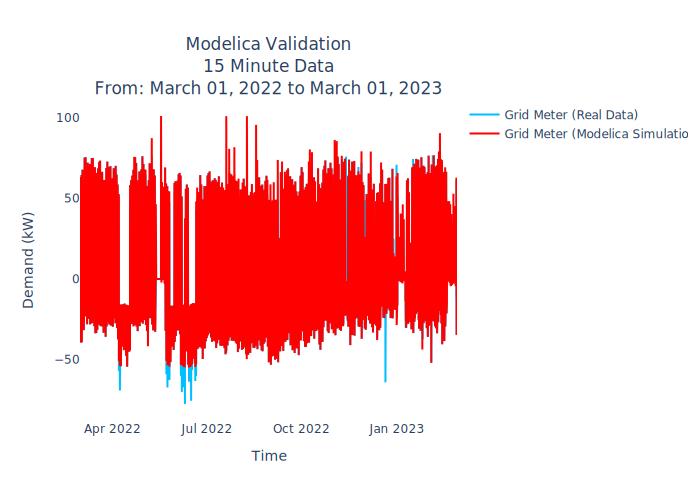
\includegraphics[width=1\linewidth]{Fig/ucr_15_Minute_Data_Mar_01_2022_to_Mar_01_2023}
			\caption{Whole Year Validation}
			\label{fig:ucr15minutedatamar012022tomar012023}
		\end{figure}
		
    \subsection{Solar Generation and Building Loads}
    	The solar power in our model is based on the historical solar data from our PV array. The HVAC loads and the regular building loads are represented separately in this model but utilize the same method; they both use historical real world power data to represent their load in the system. 
    \subsection{EV Charger Loads }
   		Our model also considers transportation loads in the form of EV chargers. The EV chargers are represented as two models: Level 2 EV chargers, and Level 3 EV chargers. While other loads follow a typical daily and yearly pattern, EV loads are different since they switch on and off. Our case study microgrid has four Level 2 chargers, so it can have four ``steps'' of 7.2 kW each, while there is only one ``step'' of 50 kW with the Level 3 chargers. To generate EV loads, we use a Poisson random generator to generate the number of charge sessions in a day, the arrival times, and charging durations based on real world data. 
		\begin{figure}[H]
			\centering
			\includegraphics[width=1\linewidth]{Fig/l2_avg_day_rand_poisson_1_hour_pdf}
			\caption{Probability Density Function of the Level 2 EV Charger Validation}
			\label{fig:l2avgdayrandpoisson1hourpdf}
		\end{figure}

%   		However, the number of sessions and duration is reduced to X and Y for the Level 3 charger.  
%		\begin{figure}[H]
%			\centering
%			\includegraphics[width=1\linewidth]{Fig/l2_avg_day_rand_poisson_1_hour}
%			\caption{Number of Real and Simulated Sessions}
%			\label{fig:l2avgdayrandpoisson1hour}
%		\end{figure}
		
		Historical data was collected from the Level-2 charger to determine the parameters for the Poisson random generator, following a typical daily charge pdf shown in Figure \ref{fig:l2avgdayrandpoisson1hourpdf}, and the power output of the Level 2 chargers in Figure \ref{fig:l2gpadpoissonjune}. 
		
			\begin{figure}[H]
				\centering
				\includegraphics[width=1\linewidth]{Fig/l2_g_pad_poisson_June}
				\caption{Level 2 Chargers Simulated Power Output}
				\label{fig:l2gpadpoissonjune}
			\end{figure}
%		\begin{figure}[H]
%			\centering
%			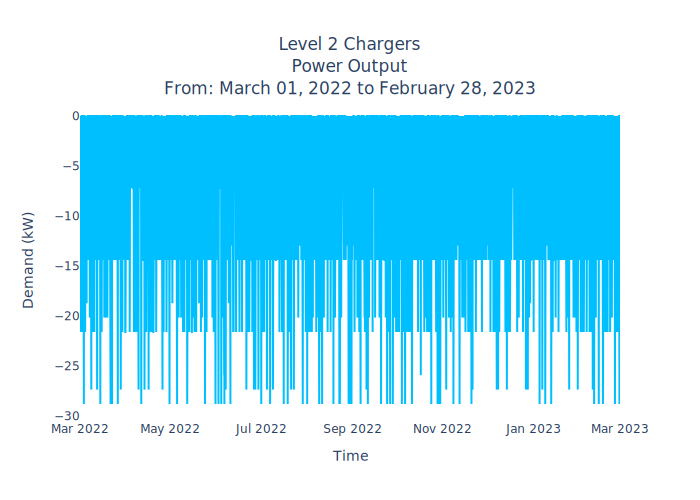
\includegraphics[width=1\linewidth]{Fig/ev_l2_po}
%			\caption{Level 2 Power Output}
%			\label{fig:evl2po}
%		\end{figure}
    
    \subsection{BESS and Peak Shaving}
    	The BESS is modeled as a battery connected to a bidirectional inverter. The BESS output is controlled by generated data from the control algorithm. The BESS output is computed in real-time by using a peak shaving algorithm utilizing  BESS SOC and the grid meter output. The algorithm charges the battery when excess solar power is exported to the grid, and the battery needs to be charged. Python code reads the net load from the grid  model and determines the amount of CO\textsubscript{2} being produced during that interval.  Algorithm \ref{alg:peakshavingflatrate} shows the peak shaving algorithm sufficient for flat rate demand response. 
%    	However,  for a TOU pricing structure, both energy and demand charges are assumed to be TOU rates with no additional flat rate demands. The TOU peak shaving algorithm is presented in Equation 1 with a simple objective to minimize the amount of power the microgrid pulls from the grid while accounting for energy and demand charges. The minimization objective is accomplished by optimizing for the summation of  TOU energy ($\Delta t \boldsymbol{\alpha}^{\boldsymbol{T}} \boldsymbol{P}^G$) and the maximums TOU demands ($\max \left(\boldsymbol{\beta}^{\text {On }} \boldsymbol{P}^G\right)+\max \left(\boldsymbol{\beta}^{\text {Mid }} \boldsymbol{P}^G\right)+\max \left(\boldsymbol{\beta}^{\text {Off }} \boldsymbol{P}^G\right)$). This algorithm is further described and validated in \cite{hasan2023universal},  \cite{hasan2021comprehensive} . \\
%%		\begin{figure}
%%			\centering
%%			\includegraphics[width=0.7\linewidth]{Fig/peak_shaving_flat_rate}
%%			\caption{Flat Rate Peak Shaving Algorithm Flowchart}
%%			\label{fig:peakshavingflatrate}
%%		\end{figure}
%			\normalsize
%			\footnotesize
%		\begin{equation} 
%			\min f\left(\boldsymbol{P}^G\right)=\Delta t \boldsymbol{\alpha}^{\boldsymbol{T}} \boldsymbol{P}^G+\max \left(\boldsymbol{\beta}^{\text {On }} \boldsymbol{P}^G\right)+\max \left(\boldsymbol{\beta}^{\text {Mid }} \boldsymbol{P}^G\right)+\max \left(\boldsymbol{\beta}^{\text {Off }} \boldsymbol{P}^G\right)
%		\end{equation}
%		\normalsize
%		subject to
%		$$
%		\begin{aligned}
%			& E_{t+1}^B=E_t^B+P_t^B \cdot \Delta t, \forall t \in \boldsymbol{T}^{\mathbf{t o t}} \\
%			& E^{B m i n} \leq E_t^B \leq E^{B m a x}, \forall t \in \boldsymbol{T}^{\mathbf{t o t}} \\
%			& P_t^B=P_t^{B+}-P_t^{B-}, \forall t \in \boldsymbol{T}^{\text {tot }} \\
%			& 0 \leq P_t^{B+} \leq \delta_t P^{B+\max }, \forall t \in \boldsymbol{T}^{\mathbf{t o t}} \\
%			& 0 \leq P_t^{B-} \leq\left(1-\delta_t\right) P^{B-\max }, \forall t \in \boldsymbol{T}^{\mathbf{t o t}} \\
%			& 0 \leq \delta_t \leq 1, \forall t \in \boldsymbol{T}^{\mathbf{t o t}} \\
%			& P_t^{B+}=\eta^{+} P_t^{S B}, \forall t \in \boldsymbol{T}^{\mathbf{t o t}} \\
%			& P_t^S=P_t^{S B}+P_t^{S L}, \forall t \in \boldsymbol{T}^{t o t} \\
%			& P_t^L=P_t^{S L}+P_t^{B L}+P_t^G, \forall t \in \boldsymbol{T}^{\text {tot }} \\
%			& P_t^{B L}=\eta^{-} P_t^{B-}, \forall t \in \boldsymbol{T}^{t o t} \\
%			& P_t^{S L} \geq 0, \forall t \in \boldsymbol{T}^{t o t}
%		\end{aligned}
%		$$

		\begin{algorithm}
			net\_load, SOC $\gets$ Modelica Data Output
			\uIf{if condition}{net\_load  <=   -15 kW and SOC > 20 \%  and net\_load  >=  -100 kW
				BESS\_inverter = -net\_load  - 15 kW
			}
			\uElseIf{net\_load  <= -100 kW and SOC > 20 \%}{
					BESS\_inverter = -100 kW
			}
			\uElseIf{net\_load  >=  0 kW and SOC < 90 \%  and net\_load  <=  100 kW}{ 
				 BESS\_inverter = -net\_load
			}
			\uElseIf{net\_load  >=  0 kW and SOC < 90 \%  }{
				 BESS\_inverter = 100 kW
			}
			\Else{
				BESS\_inverter = 0
			}
			\caption{Peak Shaving}
			\label{alg:peakshavingflatrate}
		\end{algorithm}
%		\begin{algorithm}
%			\caption{Flat Rate Peak-Shaving}}\label{alg:peak_shaving}
%			df $\gets$ dataset \\
%			output $\gets$ [] \\
%			count $\gets$ 0 \\
%			delay $\gets$ 15 minutes \\
%			new\_interval $\gets$ current\_time \\
%			\uIf {data\_length $>$ count}{
%			}
%			\uElseIf{}{
%			}	
%			\uElseIf{}{
%			}	
%			\uElseIf{}{
%			}
%			\Else{
%			}	
%		\end{algorithm}
	
\section{Results}
%    \subsection{Scenarios}

%    	\subsubsection{Scenario 1}   		
%    					\begin{figure*}
%    			\centering
%    			\begin{subfigure}[b]{0.475\textwidth}
%    				\centering
%    				\includegraphics[width=\textwidth]{Fig/ucr_theortical_actual_net_load_11_20.pdf}
%    				\caption[Network2]%
%    				{{\small UCR Microgrid Building Theoretical and Actual Load Data }}    
%    				\label{ucr_act}
%    			\end{subfigure}
%    			\hfill
%    			\begin{subfigure}[b]{0.475\textwidth}  
%    				\centering 
%    				\includegraphics[width=\textwidth]{Fig/ucr_theortical_actual_net_load_resample_11_20.pdf}
%    				\caption[]%
%    				{{\small UCR Microgrid Building Theoretical and Actual Load 15 Minute Average Resample}}    
%    				\label{ucr_act_rs}
%    			\end{subfigure}
%    			\vskip\baselineskip
%    			
%    			\caption[ The average and standard deviation of critical parameters ]
%    			{\small UCR Microgrid Building Theoretical and Actual Load} 
%    			\label{fig:ucr_act}
%    		\end{figure*}

%		\begin{figure*}
%				\begin{subfigure}[b]{0.475\textwidth}
%					\centering
%					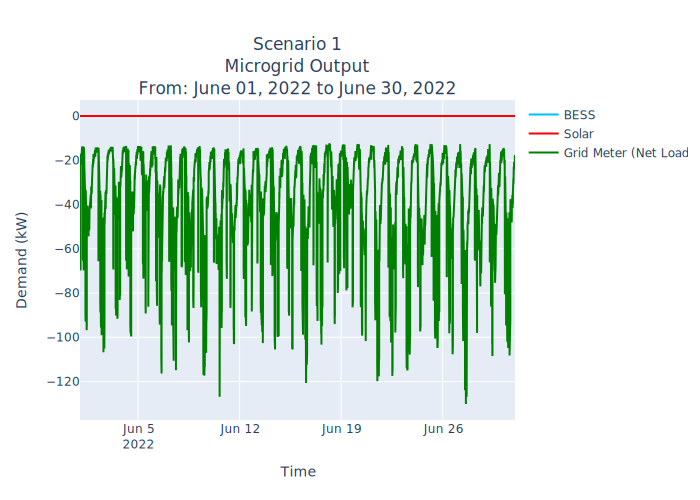
\includegraphics[width=1\linewidth]{Fig/3_Scenario_1_Mg_Output_Jun_01_2022_to_Jun_30_2022}
%					\caption{Scenario 1}
%					\label{fig:3scenario1mgoutputjun012022tojun302022}
%				\end{subfigure}
%				\hfill
%				\begin{subfigure}[b]{0.475\textwidth}
%					\centering
%					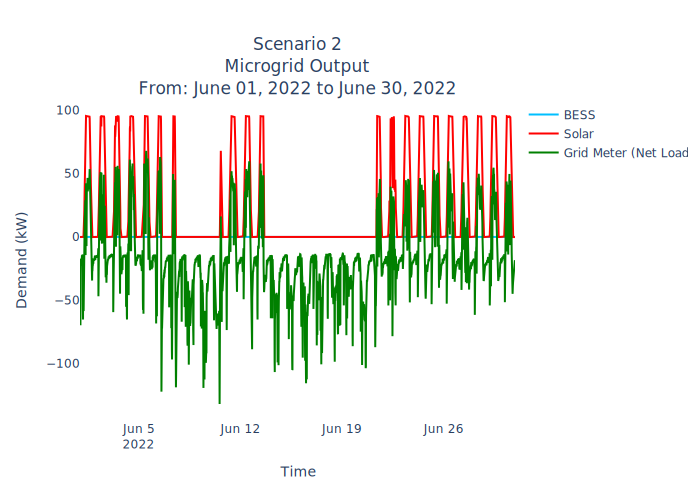
\includegraphics[width=1\linewidth]{Fig/3_Scenario_2_Mg_Output_Jun_01_2022_to_Jun_30_2022}
%					\caption{Scenario 2}
%					\label{fig:3scenario2mgoutputjun012022tojun302022}
%				\end{subfigure}			
%				
%				\begin{subfigure}[b]{0.475\textwidth}
%					\centering
%					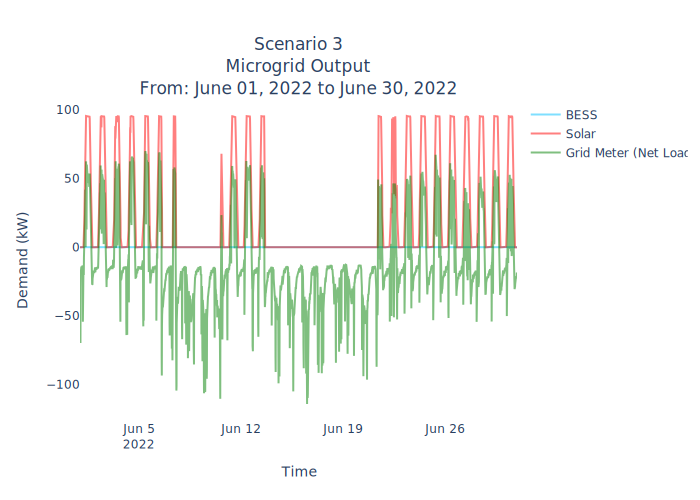
\includegraphics[width=1\linewidth]{Fig/3_Scenario_3_Mg_Output_Jun_01_2022_to_Jun_30_2022}
%					\caption{Scenario 3}
%					\label{fig:3scenario3mgoutputjun012022tojun302022}
%				\end{subfigure}
%				\hfill
%				\begin{subfigure}[b]{0.475\textwidth}
%					\centering
%					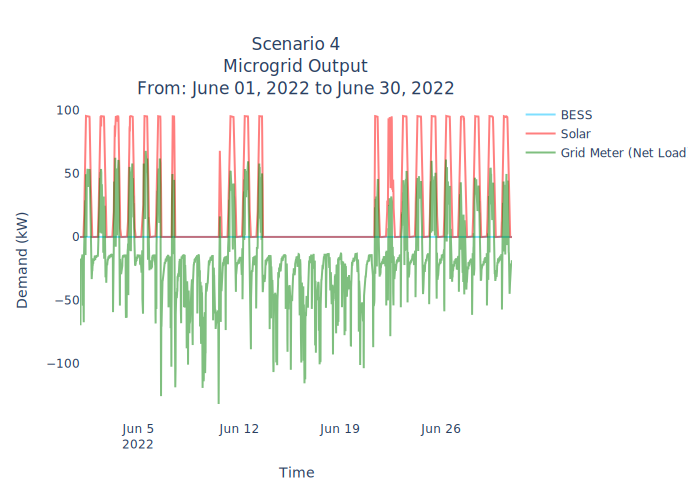
\includegraphics[width=1\linewidth]{Fig/3_Scenario_4_Mg_Output_Jun_01_2022_to_Jun_30_2022}
%					\caption{Scenario 4}
%					\label{fig:3scenario4mgoutputjun012022tojun302022}
%				\end{subfigure}				
%				
%				\begin{subfigure}[b]{0.475\textwidth}
%					\centering
%					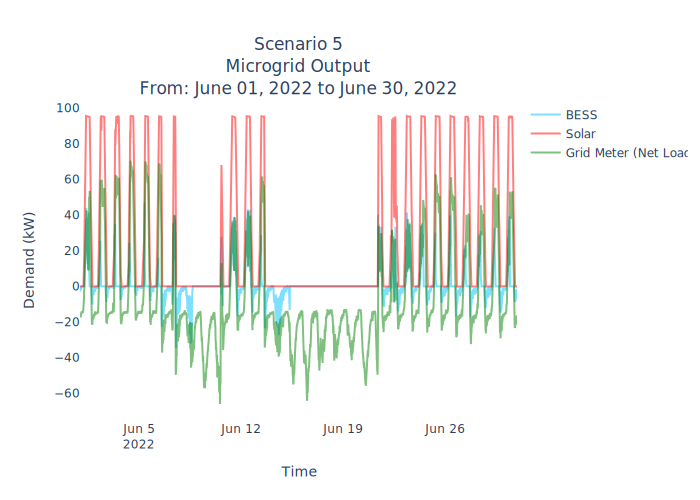
\includegraphics[width=1\linewidth]{Fig/3_Scenario_5_Mg_Output_Jun_01_2022_to_Jun_30_2022}
%					\caption{Scenario 5}
%					\label{fig:3scenario5mgoutputjun012022tojun302022}
%				\end{subfigure}				
%				\hfill
%				\begin{subfigure}[b]{0.475\textwidth}
%					\centering
%					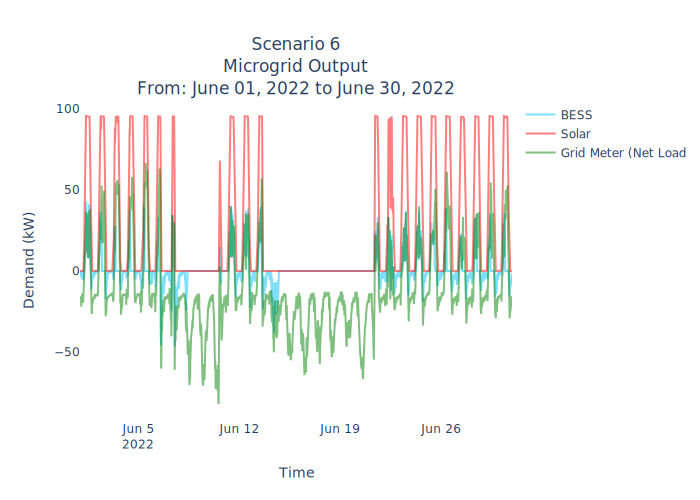
\includegraphics[width=1\linewidth]{Fig/3_Scenario_6_Mg_Output_Jun_01_2022_to_Jun_30_2022}
%					\caption{Scenario 6}
%					\label{fig:3scenario6mgoutputjun012022tojun302022}
%				\end{subfigure}
%		\end{figure*}
%				
%				\begin{figure}[H]
%					\centering
%					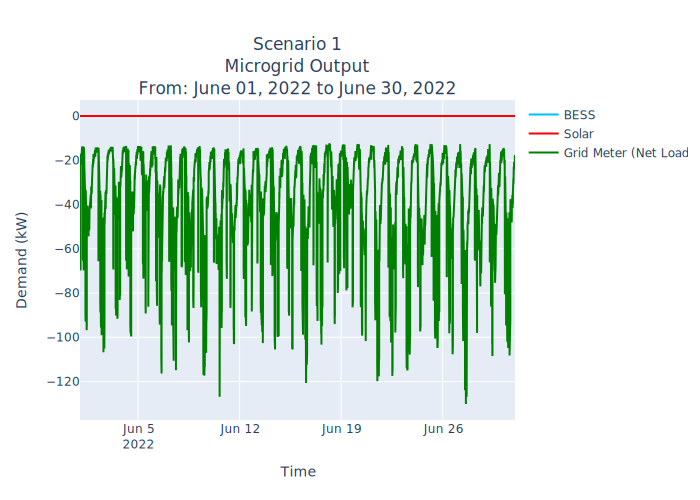
\includegraphics[width=1\linewidth]{Fig/3_Scenario_1_Mg_Output_Jun_01_2022_to_Jun_30_2022}
%					\caption{Scenario 1}
%					\label{fig:3scenario1mgoutputjun012022tojun302022}
%				\end{figure}
%				
%				\begin{figure}[H]
%					\centering
%					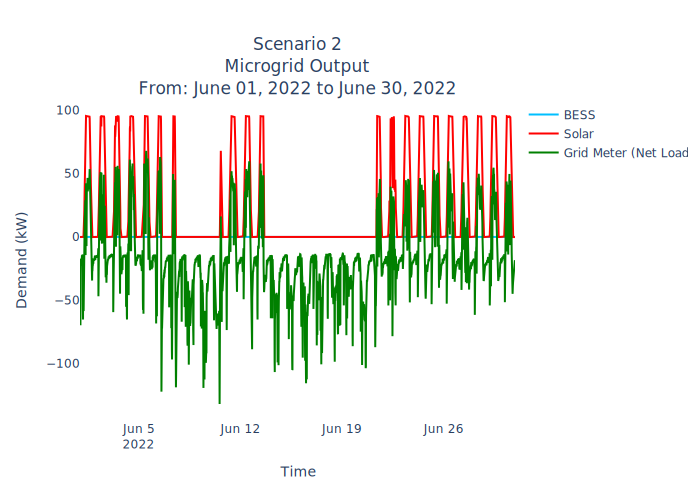
\includegraphics[width=1\linewidth]{Fig/3_Scenario_2_Mg_Output_Jun_01_2022_to_Jun_30_2022}
%					\caption{Scenario 2}
%					\label{fig:3scenario2mgoutputjun012022tojun302022}
%				\end{figure}			
%				
%				\begin{figure}[H]
%					\centering
%					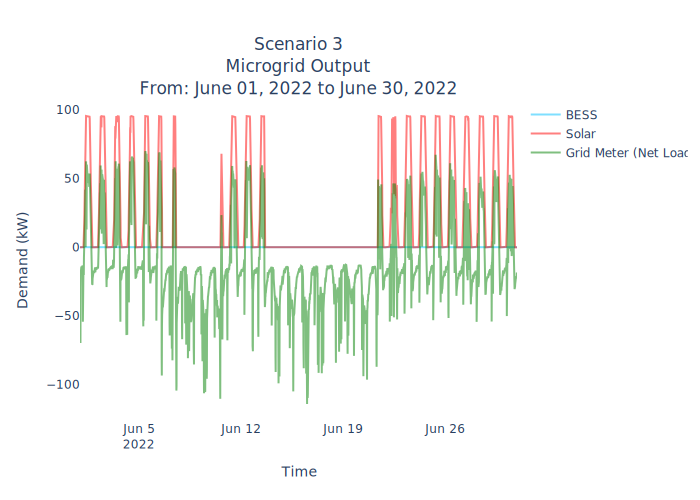
\includegraphics[width=1\linewidth]{Fig/3_Scenario_3_Mg_Output_Jun_01_2022_to_Jun_30_2022}
%					\caption{Scenario 3}
%					\label{fig:3scenario3mgoutputjun012022tojun302022}
%				\end{figure}
%				
%				\begin{figure}[H]
%					\centering
%					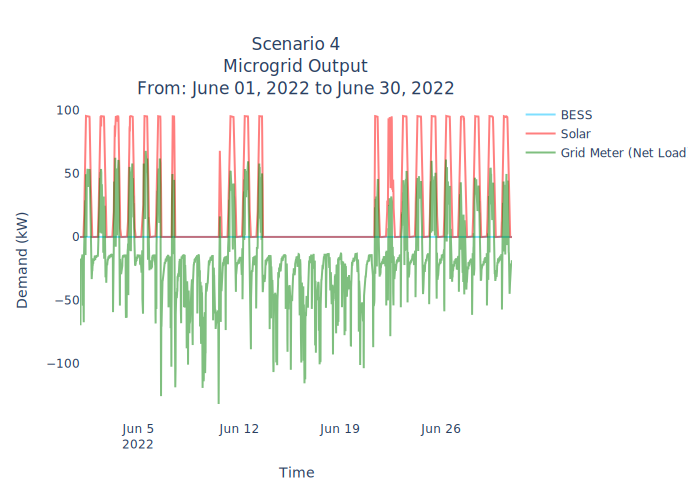
\includegraphics[width=1\linewidth]{Fig/3_Scenario_4_Mg_Output_Jun_01_2022_to_Jun_30_2022}
%					\caption{Scenario 4}
%					\label{fig:3scenario4mgoutputjun012022tojun302022}
%				\end{figure}				
%				
%				\begin{figure}[H]
%					\centering
%					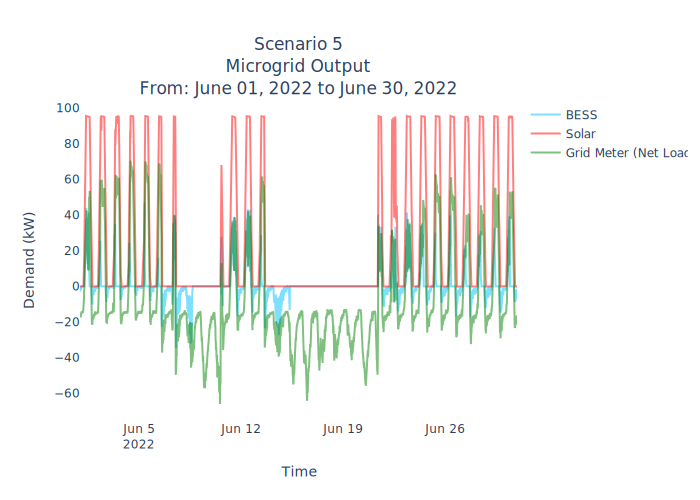
\includegraphics[width=1\linewidth]{Fig/3_Scenario_5_Mg_Output_Jun_01_2022_to_Jun_30_2022}
%					\caption{Scenario 5}
%					\label{fig:3scenario5mgoutputjun012022tojun302022}
%				\end{figure}				
%				
%				\begin{figure}[H]
%					\centering
%					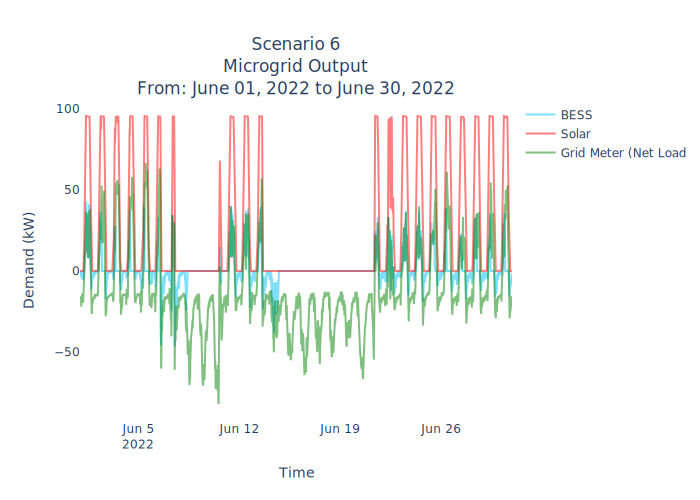
\includegraphics[width=1\linewidth]{Fig/3_Scenario_6_Mg_Output_Jun_01_2022_to_Jun_30_2022}
%					\caption{Scenario 6}
%					\label{fig:3scenario6mgoutputjun012022tojun302022}
%				\end{figure}
				
				
%			\begin{figure}[H]
%				\centering
%				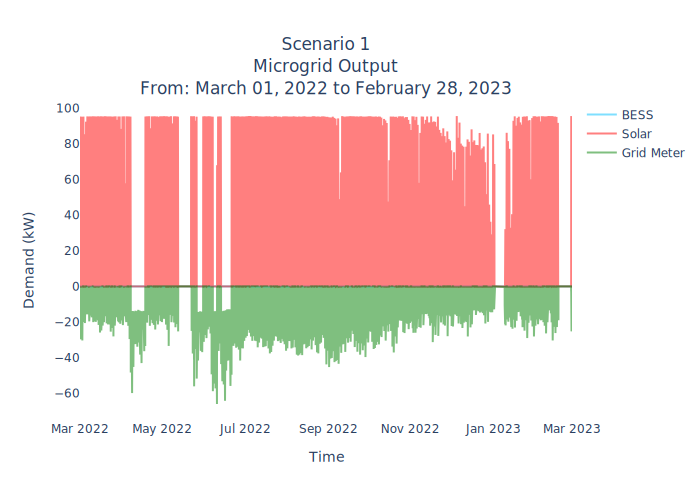
\includegraphics[width=1\linewidth]{Fig/0_Mg_Output_Mar_01_2022_to_Feb_28_2023}
%				\caption{}
%				\label{fig:0mgoutputmar012022tofeb282023}
%			\end{figure}
%    	\subsubsection{Scenario 2}
%			\begin{figure}[H]
%				\centering
%				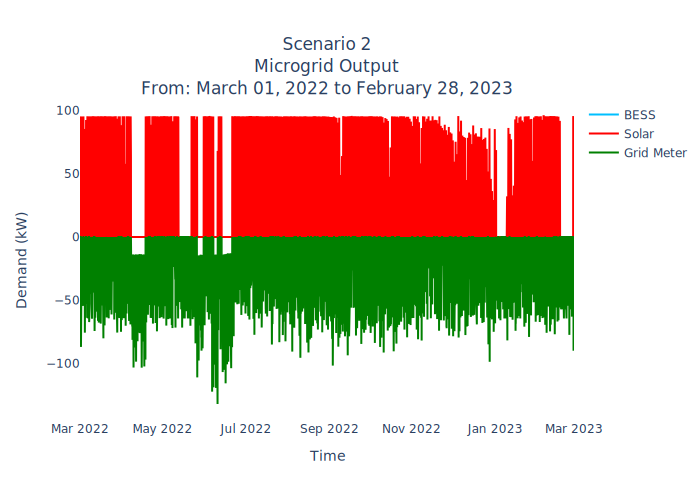
\includegraphics[width=1\linewidth]{Fig/1_Mg_Output_Mar_01_2022_to_Feb_28_2023}
%				\caption{}
%				\label{fig:1mgoutputmar012022tofeb282023}
%			\end{figure}
%    	\subsubsection{Scenario 3}
%			\begin{figure}[H]
%				\centering
%				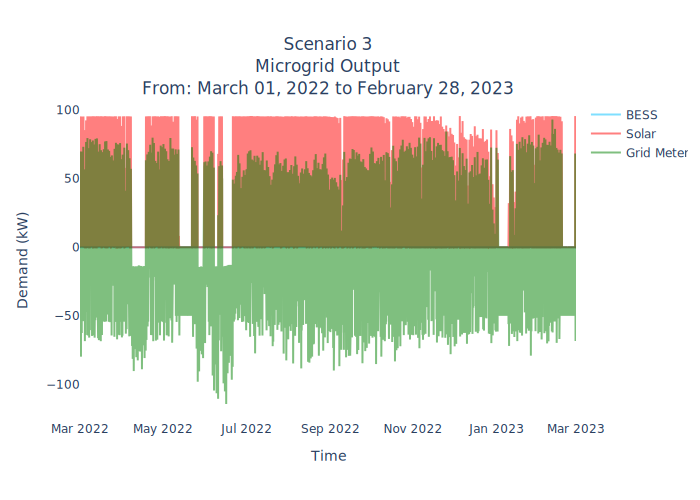
\includegraphics[width=1\linewidth]{Fig/2_Mg_Output_Mar_01_2022_to_Feb_28_2023}
%				\caption{}
%				\label{fig:2mgoutputmar012022tofeb282023}
%			\end{figure}
%    	\subsubsection{Scenario 4}
%			\begin{figure}[H]
%				\centering
%				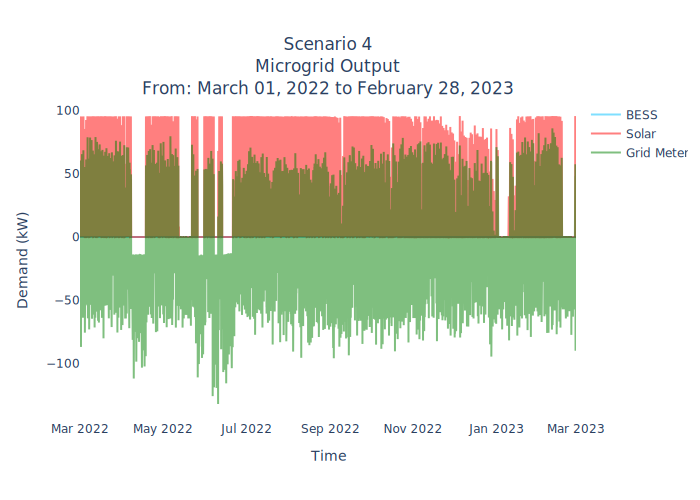
\includegraphics[width=1\linewidth]{Fig/3_Mg_Output_Mar_01_2022_to_Feb_28_2023}
%				\caption{}
%				\label{fig:3mgoutputmar012022tofeb282023}
%			\end{figure}
    		

\section{Results}
	The charging setup is modified in OpenModelica for different layouts and scenarios. The scenarios are described in Table \ref{tab:scenarios}. Scenarios 1 through 4 need to utilize the best represent a more typical setup at most EV charging stations. Scenarios 5 through 8 utilize the peak shaving abilities of a large BESS to mitigate the impacts on demand and emissions of EV charging, especially Level 3 charging. Scenarios 1 and 5 show a base case where only solar or solar and ABS are installed at a building. This is to control the experience and compare it with the other scenarios to show the impact of EV charging. scenarios 2 and 6 would be considered the more typical EV charging setup. Most commercial centers mostly use level 2 charging, which is relatively cheap and simple to install and does not have too much of a major impact. Scenarios 3,4,7,8 add one 50 kW charger to the setup. This represents the rapid adoption of fast charging and its impacts on commercial buildings.   Each scenario is run independently of one other, and the power outputs of the different components in the simulation are shown in Figure 5. Each scenario’s power pulled from the grid is juxtaposed in Figure \ref{fig:netloadscenariocomparisonsummer} and the daily CO2 emissions average from each scenario is shown in Figure \ref{fig:emissionsscenariocomparison}. The emissions and electric price amounts of each scenario are shown in Table \ref{tab:emissions}. 

%	The microgrid is modified in open Modelica for layout and scenarios. The scenarios are described in Table \ref{tab:scenarios}. Scenarios 1 and 2 are modified in open Modelica directly by shutting down both the solar system and the BESS in scenario 1 and shutting off the BESS in scenario 2. Scenarios 3 -6 by modifying the Python control algorithm open Modelica calls for the BESS. Scenario 3 represents the microgrid's current flat rate pricing structure, while scenarios 4-6 represent different optimizations if our microgrid were under different TOU rates. Each scenario is run independently of one another, and the power outputs of the different components in the simulation are shown in Figure \ref{fig:scenariosubplot}.
%%	 \ref{fig:3scenario1mgoutputjun012022tojun302022}, \ref{fig:3scenario2mgoutputjun012022tojun302022}, \ref{fig:3scenario3mgoutputjun012022tojun302022}, \ref{fig:3scenario4mgoutputjun012022tojun302022}, \ref{fig:3scenario5mgoutputjun012022tojun302022}, \ref{fig:3scenario6mgoutputjun012022tojun302022}. 
%	 Each scenario's power pulled from the grid is juxtaposed in Figure \ref{fig:netloadscenariocomparisonsummer}, and the daily CO\textsubscript{2} emissions average from each scenario is shown in Figure \ref{fig:emissionsscenariocomparison}. The emissions and electric price amount of each scenario is shown in \ref{tab:emissions}. The CO\textsubscript{2} emissions savings has scenario 1 as a reference since there is no locally-produced renewable energy in this scenario. 
	     	\begin{table}[H]
	 	\caption{Simulated Scenarios of the UCR Microgrid using Different Layouts and Electric Pricing Structures}
	 	\tiny
	 	\begin{tabularx}{\linewidth}{X | l}
\toprule
 Scenario &  \\
\midrule
		1  & No EV Charging with no BESS \\
        2 & Level 2 Charging with no BESS  \\
        3 & Level 3 Charging with no BESS  \\
        4 & Level 2 and Level 3 Charging with no BESS \\
        5 & No EV Charging with BESS \\
        6 & Level 2 Charging with BESS  \\
        7 & Level 3 Charging with BESS \\
        8 & Level 2 and Level 3 Charging with no BESS \\
\bottomrule
\end{tabularx}

	 	\normalsize
	 	\label{tab:scenarios}
	 \end{table}
	 
	 \begin{figure*}
	 	\centering
	 	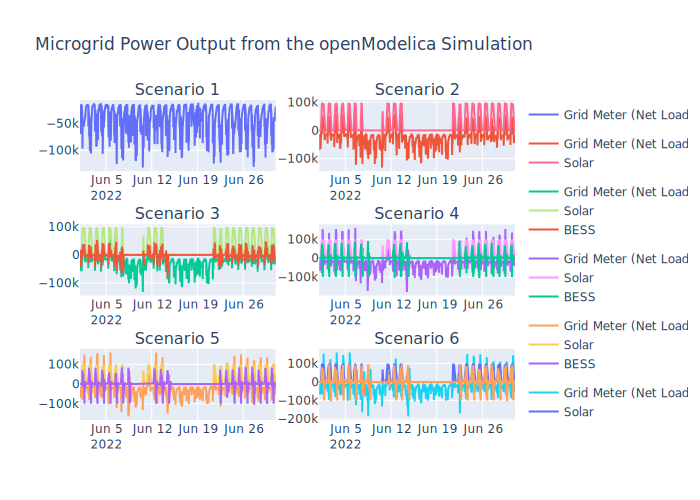
\includegraphics[width=0.9\linewidth]{Fig/scenario_subplot}
	 	\caption{openModelica Power Simulations}
	 	\label{fig:scenariosubplot}
	 \end{figure*}
	
	\begin{table}[H]
		\caption{Microgrid Utility Prices and CO\textsubscript{2} Emissions Output under Different Pricing Scenarios and Pricing Structures}
		\tiny
		\centering
		\resizebox{\columnwidth}{!}{%
		\begin{tabular}{rrrr}
\toprule
 Scenario &  Demand Charges &  Energy Charges &  Emissions \\
\midrule
        1 &            6171 &               0 &         21 \\
        2 &            7963 &            2147 &         25 \\
        3 &           12816 &            2749 &         26 \\
        4 &           14438 &            7274 &         30 \\
        5 &            4992 &               0 &         19 \\
        6 &            6755 &            2925 &         22 \\
        7 &           12053 &            4149 &         23 \\
        8 &           13109 &            8822 &         26 \\
\bottomrule
\end{tabular}

	}
		\normalsize
		\label{tab:emissions}
	\end{table}
	
%     \begin{itemize}
%        \item Pricing table under 4 methods 
%        \item Emissions table under 4 different methods 
%        \item Discuss ideal scenarios under different methods
%        \item Discuss future control methods
%    \end{itemize}   
    
	\begin{figure}[H]
		\centering
		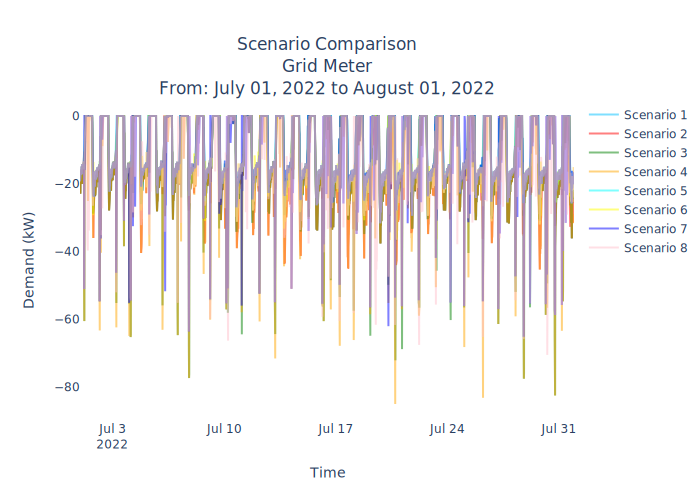
\includegraphics[width=1\linewidth]{Fig/net_load_scenario_comparison_summer}
		\caption{Summer Net Load Scenario Comparison}
		\label{fig:netloadscenariocomparisonsummer}
	\end{figure}
%	\begin{figure}[H]
%		\centering
%		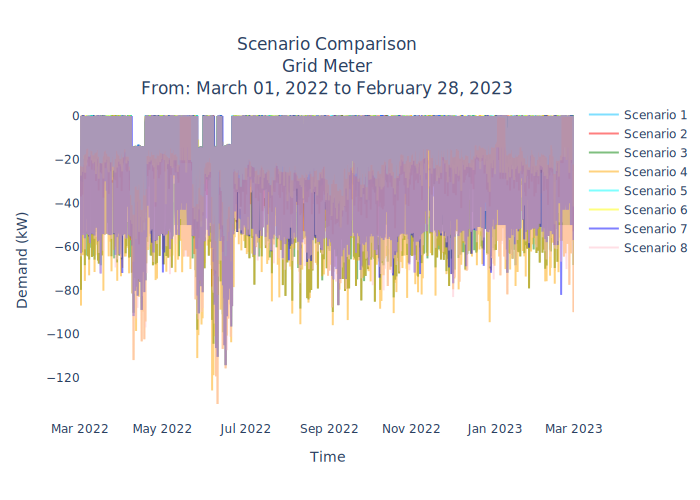
\includegraphics[width=1\linewidth]{Fig/net_load_scenario_comparison}
%		\caption{}
%		\label{fig:netloadscenariocomparison}
%	\end{figure}
	\begin{figure}[H]
		\centering
		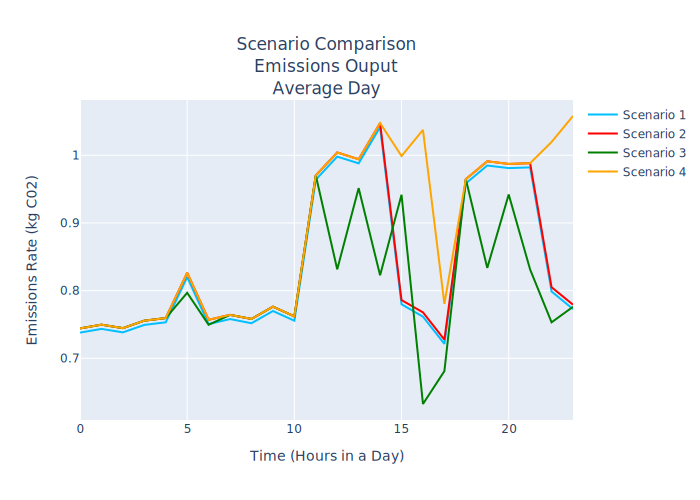
\includegraphics[width=1\linewidth]{Fig/emissions_scenario_comparison}
		\caption{Microgrid  CO\textsubscript{2} Emissions Outputs Averages During Times of Day}
		\label{fig:emissionsscenariocomparison}
	\end{figure}
	\section{Conclusion}
		Electric vehicle charging will have a significant impact on the electric costs and emission levels of a microgrid. Level 2 charging had and relatively minimal effect on costs, with a 60 to 90\% increase in electricity costs, which is not much considering that four Level 2 chargers were used. However, just one Level 3 EV charger can cause double to quadruple electric costs. Level 2 chargers have a very small impact on demand charges even when all four chargers are running since the 7.2 kilowatts of each EV charger is way less, and each has a max peak relative to the system. However, the 50 kW peaks created by the Level 3 charger nearly eclipse the demand for the HVAC units, and both  used in unisoncan double the maximum peak and the demand costs. This happens mostly at noon when HVACs and EVs run simultaneously. Energy charges for both with and without the BESS are similar, albeit slightly higher with BESS. This was expected since BESS does not reduce energy costs, only demand charges with the flat rate used by the university’s utility company. Level 2 charging and significantly easier to recover the charging costs compared to Level 3 charging. The difficulty is that just one charging event that aligns with the other loads can easily double the price of that month’s electrical bill. Implementing a Level 3 charging control system must prohibit users from utilizing fast charging at peak hours when charging one vehicle can cause major costs to the provider. Aside from the major cost differences, locally produced solar combined with EV charging has a huge potential to reduce CO2 emissions from transportation. Even when utilizing both Level 2 and three chargers and no BESS, there’s only a 42\% increase and carbon dioxide emissions compared to no EV charging at all, Increasing volume from 21 tons of CO2 to 30 tons of CO2. The X amount of vehicle trips mitigates this slight increase in CO2 if combustion engine vehicles were used instead.
	\section{Future Works}
%	Future papers will investigate different microgrid setups and optimizations for a more in-depth analysis.  The effects NEM 3.0 will have on pricing and CO\textsubscript{2} emissions compared to NEM 2.0 is of great interest. Also control algorithms and electric utility TOU rates that can optimize pricing and CO\textsubscript{2} emissions will also be assessed. 
%		\nocite{*}
		\bibliographystyle{IEEEtran}
		\bibliography{cite}
		
\end{document}
